\documentclass[12pt, titlepage]{article}

\usepackage{booktabs}
\usepackage{tabularx}
\usepackage{graphicx}
\usepackage{longtable}
\usepackage{comment}
\usepackage{siunitx}
\usepackage{afterpage}
\usepackage{pdflscape}
\usepackage{hyperref}
\hypersetup{
    colorlinks,
    citecolor=black,
    filecolor=black,
    linkcolor=red,
    urlcolor=blue
}
\usepackage[round]{natbib}
\usepackage{xr}

%% Comments

\usepackage{color}

\newif\ifcomments\commentstrue

\ifcomments
\newcommand{\authornote}[3]{\textcolor{#1}{[#3 ---#2]}}
\newcommand{\todo}[1]{\textcolor{red}{[TODO: #1]}}
\else
\newcommand{\authornote}[3]{}
\newcommand{\todo}[1]{}
\fi

\newcommand{\wss}[1]{\authornote{blue}{SS}{#1}}
\newcommand{\an}[1]{\authornote{magenta}{Author}{#1}}


%% Common Parts

\newcommand{\progname}{SSP} % PUT YOUR PROGRAM NAME HERE %Every program
                                % should have a name


\externaldocument[SRS-]{../SRS/SRS}
\newcommand{\rref}[1]{R\ref{#1}}
\newcommand{\nfrref}[1]{NFR\ref{#1}}

\externaldocument[MG-]{../Design/MG/MG}
\newcommand{\mref}[1]{M\ref{#1}}

\externaldocument[SVnV-]{../VnVPlan/SystVnVPlan/SystVnVPlan}
\newcommand{\tcref}[1]{TC\ref{#1}}

\externaldocument[UVnV-]{../VnVPlan/UnitVnVPlan/UnitVnVPlan}
\newcommand{\utcref}[1]{TC\ref{#1}}

\begin{document}

\title{Test Report: Slope Stability analysis Program (\progname{})} 
\author{Brooks MacLachlan}
\date{\today}
	
\maketitle

\pagenumbering{roman}

\section{Revision History}

\begin{tabularx}{\textwidth}{p{3cm}p{2cm}X}
\toprule {\bf Date} & {\bf Version} & {\bf Notes}\\
\midrule
12/09/18 & 1.0 & Initial write-up of document\\
12/18/18 & 1.1 & Added a comment about relative error for float equality, which 
was forgotten in the original submission\\
\bottomrule
\end{tabularx}

~\newpage

\section{Symbols, Abbreviations and Acronyms}

The symbols, abbreviations, and acronyms used in this document include those 
defined in the table below, as well as any defined in the tables found in 
Section~\ref{SRS-sec_RefMat} of the Software Requirements Specification (SRS) 
document.
\newline

\renewcommand{\arraystretch}{1.2}
\begin{tabular}{l l} 
	\toprule		
	\textbf{symbol} & \textbf{description}\\
	\midrule
	MIS & Module Interface Specification\\
	MG & Module Guide\\
	TC & Test Case\\
	VnV & Verification and Validation\\
	\bottomrule
\end{tabular}\\

\newpage

\tableofcontents

\listoftables %if appropriate

\listoffigures %if appropriate

\newpage

\pagenumbering{arabic}

This document outlines the results of testing for \progname{}. 
Section~\ref{sec_FuncReqEval} reports on the Test Cases (TCs) for functional 
requirements and Section~\ref{sec_NonFuncReqEval} reports on the tests for 
non-functional requirements, all of which are described in the System 
Verification and Validation (VnV) Plan for this project. 
Section~\ref{sec_Comparison} compares this implementation of \progname{} to the 
original implementation. Section~\ref{sec_UnitTests} reports on the results of 
the unit tests, which are described in the Unit VnV Plan for this project. 
Section~\ref{sec_Changes} comments on changes to the project that that came as 
a result of the testing. Section~\ref{sec_AutoTests} describes how the tests 
were implemented with an automated testing framework. 
Sections~\ref{sec_TraceReq} and \ref{sec_TraceMod} show the traceability 
between test cases and requirements and modules. Supporting documents and other 
resources, such as the VnVPlans and original implementation, can be found on 
\href{https://github.com/smiths/caseStudies/tree/master/CaseStudies/ssp}{the 
GitHub repository for this project}.

\section{Functional Requirements Evaluation} \label{sec_FuncReqEval}

The System VnV Plan described \tcref{SVnV-TC_InvalidSlopeNonMonotonic} - 
\tcref{SVnV-TC_InvalidUnitWtWaterNegative} for testing the requirement for 
verifying that inputs meet physical constraints. All of these tests passed. 

~\newline \noindent The next test in the System VnV Plan, \tcref{SVnV-TC_Ex1FS} 
verified 
the calculation of the factor of safety by comparing it to literature sources 
for a common example problem. The factor of safety calculated by \progname{} 
for 
this example problem was 1.3200. The average relative errors between 
\progname{} 
and each literature source are shown in Table~\ref{Table:LitFS}. The factor of 
safety calculated by \progname{} was within 1 percent of all but one of the 
literature sources. The relative tolerance was retroactively set as 0.1 for 
these tests to pass. Note that this test originally failed due to a bug for the 
case where there was no water table, which is discussed further in 
Section~\ref{sec_Changes}.

\begin{table}[!h]
\begin{tabularx}{1.0\textwidth}{p{7cm} l l}
	\toprule \textbf{Source} & \textbf{Factor of Safety} & \textbf{Relative 
	Error}\\ \midrule
	\cite{Greco1996} & 1.3270 & 0.0086\\
	\cite{MalkawiEtAl} & 1.2380 & 0.063\\
	\cite{ChengEtAl} & 1.3250 & 0.0071\\
	\cite{LiEtAl} & 1.3270 & 0.0086\\
	\bottomrule
\end{tabularx}
\caption{Relative error between \progname{} and literature for calculation of 
factor of safety}
\label{Table:LitFS}
\end{table}

~\newline \noindent The next test in the System VnV Plan, 
\tcref{SVnV-TC_Ex1Slip} 
verified the determination of the critical slip surface again by comparing it 
to literature sources. The average relative errors between \progname{} and each 
literature source are shown in Table~\ref{Table:LitSlip}. The critical slip 
surface calculated by \progname{} was within 2 percent of all but one of the 
literature sources. The relative tolerance was retroactively set as 0.1 for 
these tests to pass.

\begin{table}[!h]
\begin{tabularx}{1.0\textwidth}{l p{3.5cm}}
	\toprule \textbf{Source} & \textbf{Relative Error}\\ \midrule
	\cite{Greco1996} & 0.013\\
	\cite{MalkawiEtAl} & 0.072\\
	\cite{ChengEtAl} & 0.013\\
	\cite{LiEtAl} & 0.013\\
	\bottomrule
\end{tabularx}
\caption{Relative error between \progname{} and literature for calculation of 
critical slip surface}
\label{Table:LitSlip}
\end{table}

~\newline \noindent The next test in the System VnV Plan, 
\tcref{SVnV-TC_OrigProgFS} 
verified the calculation of the factor of safety by comparing it to the 
original implementation for a specific example. The factor of safety calculated 
by \progname{} for this example problem was 0.9808, compared to 0.9835 for the 
original program. The average relative error between \progname{} and the 
original 
program was 0.0027. The relative tolerance was retroactively set as 0.01 for 
these tests to pass.

~\newline \noindent The next test in the System VnV Plan, 
\tcref{SVnV-TC_OrigProgSlip} 
verified the calculation of the critical slip surface by comparing it to the 
original implementation for a specific example. The critical slip surface 
calculated by \progname{} for this example problem is shown in 
Figure~\ref{Fig:Slip}. The average relative error between \progname{} and the 
original program was 0.019 The relative tolerance was retroactively set as 0.05 
for these tests to pass.

\begin{figure}[h!]
	\begin{center}
		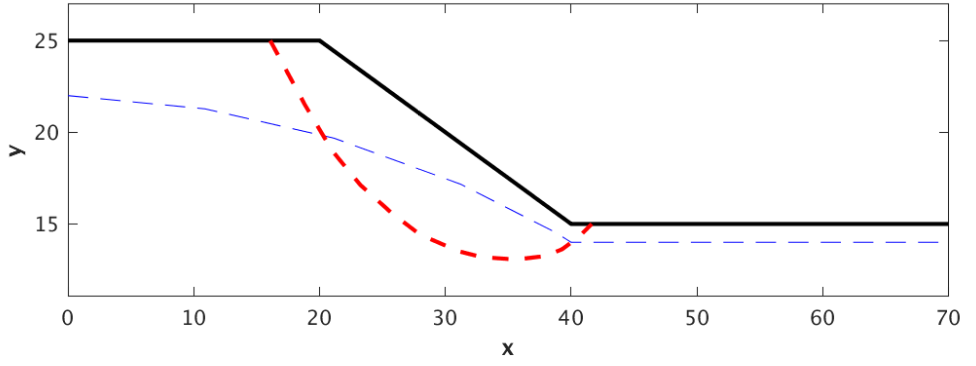
\includegraphics[width=1.0\textwidth]{Slip.png}
		\caption{The critical slip surface for \tcref{SVnV-TC_OrigProgSlip} 
			calculated by \progname{}}
		\label{Fig:Slip}
	\end{center}
\end{figure}

~\newline \noindent The next tests in the System VnV Plan, 
\tcref{SVnV-TC_OrigProgNormal} 
and \tcref{SVnV-TC_OrigProgShear} verified the calculation of the interslice 
normal and shear forces by comparing them the original implementation for a 
specific example. Originally, the relative error between the current 
implementation and the original implementation was unexpectedly high, which led 
to the discovery of a bug in the current implementation, which was then fixed. 
This is discussed further in Section~\ref{sec_Changes}. After fixing the bug, 
the test was performed again. The interslice forces calculated by \progname{} 
for 
this example problem are shown in Figure~\ref{Fig:Forces}. The average relative 
error between \progname{} and the original program was 0.099 for the normal 
forces and 0.072 for the shear forces. These relative errors were still higher 
than expected, but further investigation found that there is a high variance in 
these calculations, even in the original program. For example, the peak 
interslice normal force was seen to vary between about 140 \si{\kilo\newton} 
and 200 \si{\kilo\newton} for different runs of the original program. As a 
result, the tests were given a relatively high relative tolerance of 0.15 and 
were compared to outputs from multiple runs of the original program. As long as 
the relative error is less than the relative tolerance for at least one of the 
outputs, the tests pass. With these changes, both tests pass on the vast 
majority of runs.

\begin{figure}[h!]
	\begin{center}
		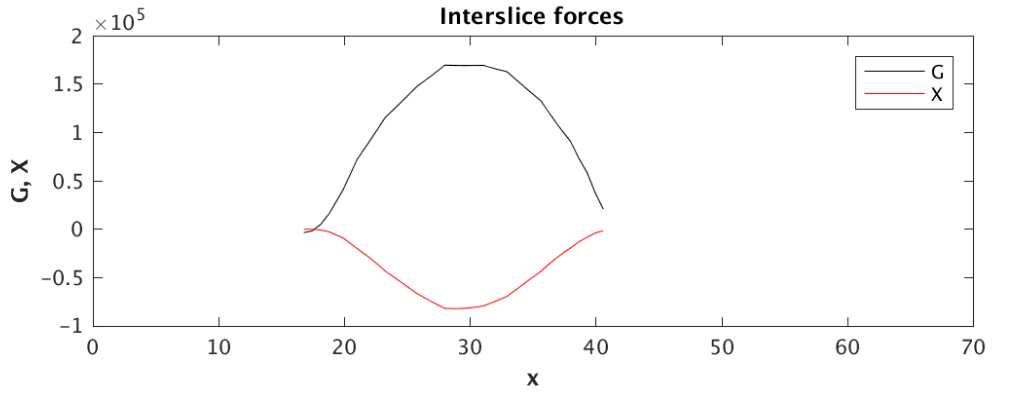
\includegraphics[width=1.0\textwidth]{Forces.png}
		\caption{The interslice normal and shear forces for  
		\tcref{SVnV-TC_OrigProgNormal} and  \tcref{SVnV-TC_OrigProgShear}
			calculated by \progname{}}
		\label{Fig:Forces}
	\end{center}
\end{figure}

~\newline \noindent The next test in the System VnV Plan, 
\tcref{SVnV-TC_CalcConstantf}, 
verified that changing the type of the function $f$ to a constant has an impact 
on the result. This was done by visual inspection of the critical slip surface 
and interslice forces for the case where \textit{const\_f} is true. These plots 
are shown in Figure~\ref{Fig:ConstF}. The factor of safety was 0.8363 for this 
test. The results were similar overall to the case where \textit{const\_f} was 
false, with some notable differences: A slightly higher exit x-value for the 
slip surface, associated with notably different interslice forces near the 
exit, and an approximately 14 percent difference in factor of safety. These 
slight differences give confidence that \progname{} actually translated the 
\textit{const\_f} input to a different $f$ function, which is what this test 
was checking for, and thus the test was considered a pass.

\begin{figure}[h!]
	\begin{center}
		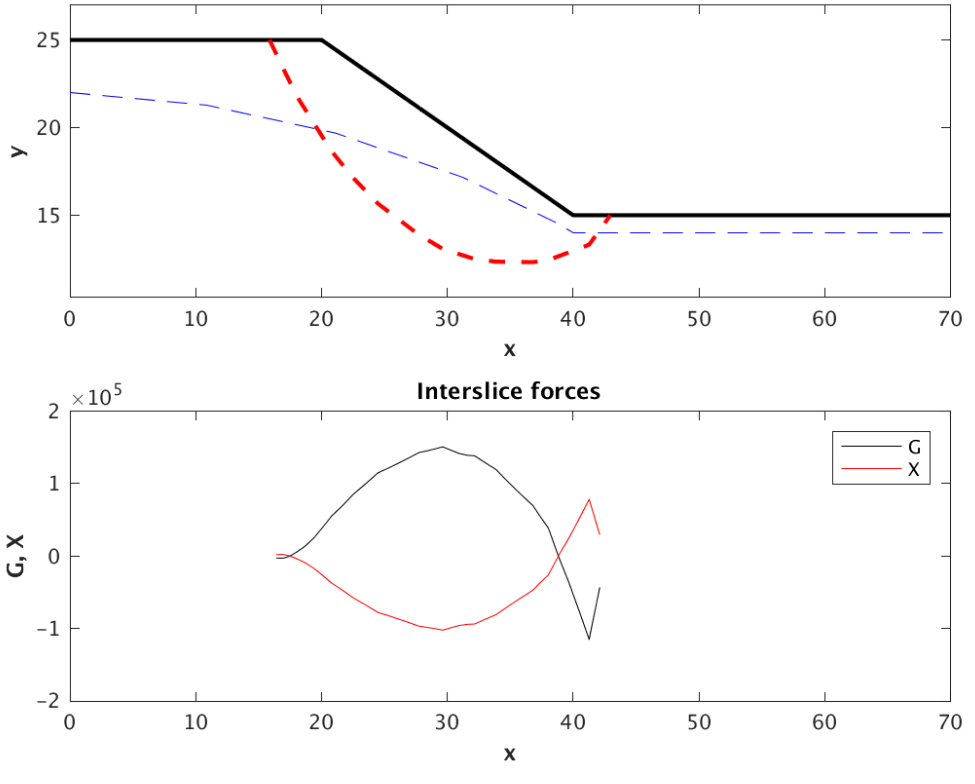
\includegraphics[width=1.0\textwidth]{ConstFPlots.png}
		\caption{The critical slip surface (top) and interslice normal and 
		shear forces (bottom) for  \tcref{SVnV-TC_CalcConstantf} calculated by 
		\progname{}}
		\label{Fig:ConstF}
	\end{center}
\end{figure}

~\newline \noindent The final functional requirement tests in the System VnV 
Plan, \tcref{SVnV-TC_OutputInputXEtrMin} - \tcref{SVnV-TC_ValidOutFS}, were for 
verifying the requirements for verifying and delivering output. These tests all 
passed.

\section{Nonfunctional Requirements Evaluation} \label{sec_NonFuncReqEval}

\subsection{Correctness}

The success of the system tests for the calculations of \progname{}, 
specfically \tcref{SVnV-TC_Ex1FS} - \tcref{SVnV-TC_OrigProgShear}, gives 
confidence in the correctness of \progname{}.

\subsection{Maintainability}

\tcref{SVnV-TC_Maintainability} in the System VnV Plan is a test for gaining 
confidence in the maintainability of \progname{}. The test question was asked 
to a volunteer test subject who was given the Module Guide (MG) for \progname{} 
as a resource to answer the question. The volunteer's response was the Input 
module, Morgenstern-Price calculation module, and potentially the Slice 
Property Calculation and Genetic Algorithm modules. This answer was correct 
with the exception of the Genetic Algorithm module. The volunteer's explanation 
for thinking this module might need to be changed was that, due to their lack 
of domain knowledge, they did not know if the changes to the Morgenstern-Price 
Calculation module would include changes to its interface. Since the Genetic 
Algorithm module uses the Morgenstern-Price Calculation module, it would need 
to be changed if the interface to the Morgenstern-Price Calculation module 
changed. This explanation was not only reasonable but also prudent, and thus 
the response was considered correct and this test result was considered a pass, 
giving confidence in the maintainability of \progname{}.
		
\subsection{Reusability}

\tcref{SVnV-TC_Reusability} in the System VnV Plan is a test for gaining 
confidence in the reusability of \progname{}. The alternative input module was 
written based off of the Input module from the previous implementation, which 
accepted some user inputs by keyboard input. This alternative Input Module is 
called ``InputKeyboard.m'' and can be found in the GitHub repository for this 
project. The current Input Module was temporarily replaced by this alternative 
Input Module. The system tests in ``control\_test.m'' were then ran. The tests 
passed, showing that all of the other modules were reusable in this alternative 
version of \progname{}.

\subsection{Understandability}
Since maintainability and reusability are related to understandability, the 
success of the tests for those requirements gives confidence in the 
understandability of \progname{}.
	
\section{Comparison to Existing Implementation} \label{sec_Comparison}

The results of \tcref{SVnV-TC_OrigProgFS} - \tcref{SVnV-TC_OrigProgShear} from 
the System VnV Plan showed how the current implementation provides similar 
results to the previous implementation, as discussed in 
Section~\ref{sec_FuncReqEval}. However, the current implementation improved 
upon the existing implementation in other regards. The existing implementation 
had tests, but they were implemented without a unit testing framework and did 
not work when the instructions for running them were followed. The tests also 
did not cover every module. The new implementation has working tests 
implemented with a unit testing framework, meaning they are easy to run and 
easy to add to in the future. Since the tests were developed in a systematic 
fashion based on the Module Interface Specification (MIS), they extensively 
cover all of the modules that are implemented by \progname{}. In addition, the 
tests uncovered an oversight in the original implementation, a case that was 
not accounted for in the code, which is discussed further in 
Sections~\ref{sec_UnitTests} and \ref{sec_Changes}.

\section{Unit Testing}  \label{sec_UnitTests}
The Unit VnV Plan described \tcref{UVnV-TC_InputSlope} - 
\tcref{UVnV-TC_OutputFile}, all of which were implemented in the unit testing 
framework and passed, with the exception of 
\tcref{UVnV-TC_SlicerNotEvnslcIndivisible}, which failed on the first run, 
revealing that the Slip Slicing module had not been properly implemented for 
the case where the desired number of slices was indivisible by the starting 
number of slices. This prompted changes to the implementation, discussed 
further in Section~\ref{sec_Changes}. The test passed after these changes. For 
tests that asserted on equality of floats, the relative errors ranged from 
about $3 \cdot 10^{12}$ to $3 \cdot 10^{11}$, so the relative tolerance was 
retroactively set as $10^{10}$ for the tests to pass.

\section{Changes Due to Testing} \label{sec_Changes}
The failure of \tcref{UVnV-TC_SlicerNotEvnslcIndivisible} revealed that the 
implementation had not considered the case where the \textit{soln.evnslc} 
variable (see MIS for more information) was false and the desired number of 
slices was not divisible by the initial number of slices. This prompted a 
change to the Slip Slicing module to properly handle this case. 

~\newline \noindent The system test \tcref{SVnV-TC_Ex1FS} initially failed, 
revealing a bug in the case where there is no water table. In this case, the 
unit weight of water was set to 0 and thus violated the constraint that it must 
be greater than 0. The implementation was changed to only enforce this 
constraint when a water table exists.

~\newline \noindent The system tests \tcref{SVnV-TC_OrigProgNormal} 
and \tcref{SVnV-TC_OrigProgShear} initially had very high relative errors, 
leading to the discovery of a bug where the interslice forces were not properly 
being mirrored in the case where expected soil motion is left-to-right. In this 
case, \progname{} is supposed to temporarily mirror the slope so that the 
direction of soil motion is right-to-left, and then mirror the slope and slip 
surface back to their original orientation before outputting the results. The 
interslice forces were not being mirrored back to the original implementation, 
leading to the addition of code to rectify this error.

\section{Automated Testing} \label{sec_AutoTests}

Every test, with the exception of \tcref{SVnV-TC_CalcConstantf} and the tests 
for non-functional requirements, was automated so that the tests could be 
executed with a simple command. This was done by implementing the tests with 
MatLab's built-in unit testing framework. MatLab provides the ``runtests'' 
function for running all of the tests in a given directory.
		
\section{Trace to Requirements} \label{sec_TraceReq}

Tables~\ref{Table:TraceTestReq} and \ref{Table:TraceTestNFReq} were taken 
directly from the System VnV Plan document for this project. It shows that the 
tests effectively cover every Requirement (R) and Non-Functional Requirement 
(NFR) from the SRS. Unless otherwise specified, the test cases referenced in 
the table refer to tests described in the System VnV Plan.

\begin{table}[!h]
	\centering
	\begin{tabular}{|c|c|c|c|c|c|c|c|c|c|c|c|}
		\hline
		& \rref{SRS-R_Inputs}& \rref{SRS-R_VerifyInput}& \rref{SRS-R_InitGen}& 
		\rref{SRS-R_FS}& \rref{SRS-R_Minimize} & \rref{SRS-R_VerifyOutput}& 
		\rref{SRS-R_OutputInputs}& \rref{SRS-R_CritGraph}& 
		\rref{SRS-R_OutputFS}& 
		\rref{SRS-R_NormalGraph}& \rref{SRS-R_ShearGraph} \\
		\hline
		UnitVnVPlan \tcref{UVnV-TC_InputSlope} - 
		\tcref{UVnV-TC_InputXMaxExtEqual}               
		& X& & & & & & & & & & \\ \hline
		\tcref{SVnV-TC_InvalidSlopeNonMonotonic} - 
		\tcref{SVnV-TC_InvalidUnitWtWaterNegative} 
		& & X& & & & & & & & & \\ \hline
		\tcref{SVnV-TC_Ex1FS} - 
		\tcref{SVnV-TC_OrigProgSlip}                             
		& & & X& X& X& & & & & & \\ \hline
		\tcref{SVnV-TC_OrigProgNormal}                                          
		    
		& & & & & & & & & X& & \\ \hline
		\tcref{SVnV-TC_OrigProgShear}                                           
		    
		& & & & & & & & & & X& \\ \hline
		\tcref{SVnV-TC_OutputInputXEtrMin} - 
		\tcref{SVnV-TC_OutputInputConstf}   
		& & & & & & & X& & & & \\ \hline
		\tcref{SVnV-TC_OutFS}                                                   
		    
		& & & & & & & & X& & & \\ \hline
		\tcref{SVnV-TC_OutSlip}                                                 
		    
		& & & & & & & & & X& & \\ \hline
		\tcref{SVnV-TC_OutNormal}                                               
		    
		& & & & & & & & & & X& \\ \hline
		\tcref{SVnV-TC_OutShear}                                                
		    
		& & & & & & & & & & & X \\ \hline
		\tcref{SVnV-TC_ValidOutFS}                   
		& & & & & & X& & & & & \\
		\hline
	\end{tabular}
	\caption{Traceability matrix showing the connections between functional 
		requirements and test cases}
	\label{Table:TraceTestReq}
\end{table}

\begin{table}[!h]
	\centering
	\begin{tabular}{|c|c|c|c|c|}
		\hline
		& \nfrref{SRS-NFR_Correctness}& \nfrref{SRS-NFR_Understandability}& 
		\nfrref{SRS-NFR_Reusability}& \nfrref{SRS-NFR_Maintainability} \\
		\hline
		\tcref{SVnV-TC_Ex1FS} - 
		\tcref{SVnV-TC_OrigProgShear}                             
		& X& & & \\ \hline
		\tcref{SVnV-TC_Maintainability}                                         
		   
		& & X& &X \\ \hline
		\tcref{SVnV-TC_Reusability}                     
		& & X& X& \\
		\hline
	\end{tabular}
	\caption{Traceability matrix showing the connections between non-functional 
		requirements and test cases}
	\label{Table:TraceTestNFReq}
\end{table}
		
\section{Trace to Modules} \label{sec_TraceMod}

Table~\ref{Table:TraceTestMod} was taken directly from the Unit VnV Plan 
document for this project, with the addition of one row for the System VnV Plan 
tests. It shows that the tests effectively cover every 
Module (M) from the MG and MIS, with the exception of those not implemented by 
\progname{}. Unless otherwise specified, the test cases referenced in the table 
refer to tests described in the Unit VnV Plan.

\afterpage{
	\begin{landscape}
		\begin{table}[!h]
			\centering
			\begin{tabular}{|c|c|c|c|c|c|c|c|c|c|c|c|c|c|}
				\hline
				& \mref{MG-mHH}& \mref{MG-mControl}& \mref{MG-mInput}& 
				\mref{MG-mGenAlg}& \mref{MG-mKinAdm} & \mref{MG-mSlipWeight}& 
				\mref{MG-mSlipSlicer}& \mref{MG-mMorgPrice}& 
				\mref{MG-mSliceProperty}& 
				\mref{MG-mOutput}& \mref{MG-mArrayOps}& \mref{MG-mRandNum}& 
				\mref{MG-mPlot} \\
				\hline
				System VnV Plan & & X& & & & & & & & & & &\\ \hline
				\tcref{UVnV-TC_InputSlope} - 
				\tcref{UVnV-TC_InputUnexpected}                 
				& & & X& & & & & & & & & & \\ \hline
				\tcref{UVnV-TC_GenAlgXextMin} - \tcref{UVnV-TC_GenAlgVertices} 
				& & & & X& & & & & & & & &\\ \hline
				\tcref{UVnV-TC_KinAdmXDec} - 
				\tcref{UVnV-TC_KinAdmObtuOff}          
				& & & & & X& & & & & & & & \\ \hline
				\tcref{UVnV-TC_WeighterSort} - 
				\tcref{UVnV-TC_WeighterLast}       
				& & & & & & X& & & & & & & \\ \hline
				\tcref{UVnV-TC_SlicerEvnslcSize} - 
				\tcref{UVnV-TC_SlicerNotEvnslcVals}
				& & & & & & & X& & & & & & \\ \hline
				\tcref{UVnV-TC_MorgPriceNonConvergingFs} - 
				\tcref{UVnV-TC_MorgPriceSpuriousX}   
				& & & & & & & & X& & & & & \\ \hline
				\tcref{UVnV-TC_PropertyWWet} - \tcref{UVnV-TC_PropertyHeight}
				& & & & & & & & & X& & & & \\ \hline
				\tcref{UVnV-TC_InvalidFs} - \tcref{UVnV-TC_OutputFile}
				& & & & & & & & & & X& & & \\
				\hline
			\end{tabular}
			\caption{Traceability matrix showing the connections between 
			modules and 
				test cases}
			\label{Table:TraceTestMod}
		\end{table}
	\end{landscape}
}

\section{Code Coverage Metrics}
Not applicable for \progname{}.

\newpage

\bibliographystyle{plainnat}

\bibliography{../../refs/References}

\end{document}